\documentclass[12pt]{article}

\usepackage[T2A]{fontenc}        % поддержка кириллицы
\usepackage[utf8]{inputenc}      % кодировка utf-8
\usepackage[russian]{babel}      % включаем русский язык
\usepackage{amsmath,amssymb}
\usepackage{geometry}
\geometry{left=2cm,right=2cm,top=2cm,bottom=2cm}
\usepackage{graphicx}            % вставка изображений
\usepackage{hyperref}
\usepackage{indentfirst}         % отступ первого абзаца в разделе 
\usepackage{minted}              % листинг кода
\usemintedstyle{perldoc}         % стиль листинга

\begin{document}

%----------------------------------------
% Титульный лист
%----------------------------------------
\begin{titlepage}
\centering
{\large Санкт-Петербургский Государственный Электротехнический Университет «ЛЭТИ»\par}
\vspace{1.5cm}
{\large кафедра физики\par}
\vspace{3cm}
{\LARGE \textbf{Задание №1 по разделу \\ «Электростатика»}\par}
\vspace{1cm}
{\Large Название: Численное решение уравнения Лапласа и построение силовой линии.\par}
\vspace{3cm}
\begin{flushright}
    \begin{tabular}{@{}r@{\quad}l@{}}
        Фамилия И.О.: & Николаев В.Ю.\\[0.5cm]
        Группа:        & 4395\\[0.5cm]
        Преподаватель: & Альтмарк А.М.\\[0.5cm]
        Итоговый балл: & \\[0.5cm]
        Крайний срок сдачи: & 17.04\\[0.5cm]
    \end{tabular}
\end{flushright}
\vfill
{\Large Санкт-Петербург 2025\par}
\end{titlepage}

%----------------------------------------
\section*{Условие задания}
Дана электростатическая система из трёх электродов. Внешний электрод потенциалом \(0\,\text{В}\), два внутренних — \(7\,\text{В}\) и \(-8\,\text{В}\) соответственно. Необходимо:
\begin{enumerate}
    \item Найти распределение потенциала \(\varphi(x,y)\) решением уравнения Лапласа \(\nabla^2\varphi=0\) в области \([-6,6]\times[-6,6]\).
    \item Построить силовую линию (кривая, касательная к вектору напряжённости \(\mathbf E=-\nabla\varphi\)) через точку \((0,-2)\).
    \item Записать длину этой линии в файл \texttt{IDZ1.txt}.
    \item Визуализировать результат: контуры электродов, карту потенциала, векторы поля и траекторию силовой линии.
\end{enumerate}

\begin{center}
\begin{tabular}{|l|l|}
\hline
Вар.: & 14 \\
Уравнение внешнего электрода: & \(x^2 + y^2 = 25\) \\
Уравнение электрода 1: & \(\tfrac{3|\tfrac95 + x|^3}{10} + \tfrac{4|y|^3}{5} = \tfrac12\) \\
Уравнение электрода 2: & \(\tfrac{|\,-\tfrac95 + x\,|^2}{2} + |y|^2 = \tfrac45\) \\
Точка силовой линии: & \((0,-2)\) \\
\hline
\end{tabular}
\end{center}

%----------------------------------------
\section*{Физическая постановка задачи}
На границе задаются потенциалы:
\[
\varphi=0\text{ на }x^2+y^2=25,\quad
\varphi=7\text{ по первому внутреннему контуру},\quad
\varphi=-8\text{ по второму внутреннему контуру}.
\]
Во внутренних точках решается
\[
\nabla^2\varphi=0.
\]
Силовая линия — интегральная кривая
\[
\frac{d\mathbf r}{ds}=-\frac{\nabla\varphi}{\|\nabla\varphi\|},
\]
начиная с \((0,-2)\) в обе стороны до достижения любого электрода.

%----------------------------------------
\section*{Метод решения}
\subsection*{Численное решение уравнения Лапласа}
Реализовано в C++ методом SOR с красно-чёрным обходом:
\[
V_{i,j}^{\text{new}}=V_{i,j}+\omega\Bigl(\tfrac{V_{i+1,j}+V_{i-1,j}+V_{i,j+1}+V_{i,j-1}}{4}-V_{i,j}\Bigr),
\]
где \(\omega=1.8\).  
Сетка \(601\times601\) на области \([-6,6]^2\), жёсткий критерий сходимости \(\|\Delta V\|_\infty<10^{-6}\).

\subsection*{Построение силовой линии}
\begin{itemize}
  \item Вычисляем градиент центра\-льными разностями, затем делаем билинейную интерполяцию.
  \item Интегрируем уравнение силовой линии с шагом \(ds=10^{-5}\) и до \(10^6\) шагов в каждую сторону:
    \[
      \mathbf r_{n+1}=\mathbf r_n - ds\;\frac{\nabla V(\mathbf r_n)}{\|\nabla V(\mathbf r_n)\|}.
    \]
  \item Останавливаемся, как только точка попадает на любой электрод (допуск \(0.05\)).
\end{itemize}

%----------------------------------------
\section*{Краткие фрагменты кода}
\subsection*{Решение методом SOR (C++)}
\begin{minted}[fontsize=\footnotesize,linenos]{cpp}
for(int pass=0; pass<2; ++pass) {
  bool updateRed = (pass==0);
  for(int j=1; j<ny-1; ++j)
    for(int i=1; i<nx-1; ++i) {
      if(fixed_mask[j*nx+i] || isRed(i,j)!=updateRed) continue;
      double sum = V[(j-1)*nx+i] + V[(j+1)*nx+i]
                 + V[j*nx+i-1] + V[j*nx+i+1];
      double diff = sum*0.25 - V[j*nx+i];
      V[j*nx+i] += omega * diff;
    }
}
\end{minted}

\subsection*{Интегратор силовой линии (C++)}
\begin{minted}[fontsize=\footnotesize,linenos]{cpp}
double ds = 1e-5;
int    maxSteps = 1000000;
auto step = [&](double &x,double &y,int sign){
  auto gx = bilinear(dVdx,xs,ys,nx,ny,x,y);
  auto gy = bilinear(dVdy,xs,ys,nx,ny,x,y);
  double norm = std::hypot(gx,gy);
  x += sign * ds * (-gx/norm);
  y += sign * ds * (-gy/norm);
};
\end{minted}

\subsection*{Визуализация (Python)}
\begin{minted}[fontsize=\footnotesize,linenos]{python}
V = np.loadtxt("data/potential.csv", delimiter=',')
path = np.loadtxt("data/fieldline.csv", delimiter=',')
# построение contourf, quiver и траектории...
\end{minted}

%----------------------------------------
\section*{Результаты и примеры работы}
После запуска C++-программы:
\begin{itemize}
  \item В папке \texttt{data/} появились файлы \texttt{potential.csv} и \texttt{fieldline.csv}.
  \item В корне проекта создан \texttt{IDZ1.txt} с длиной силовой линии.
\end{itemize}
\begin{center}
  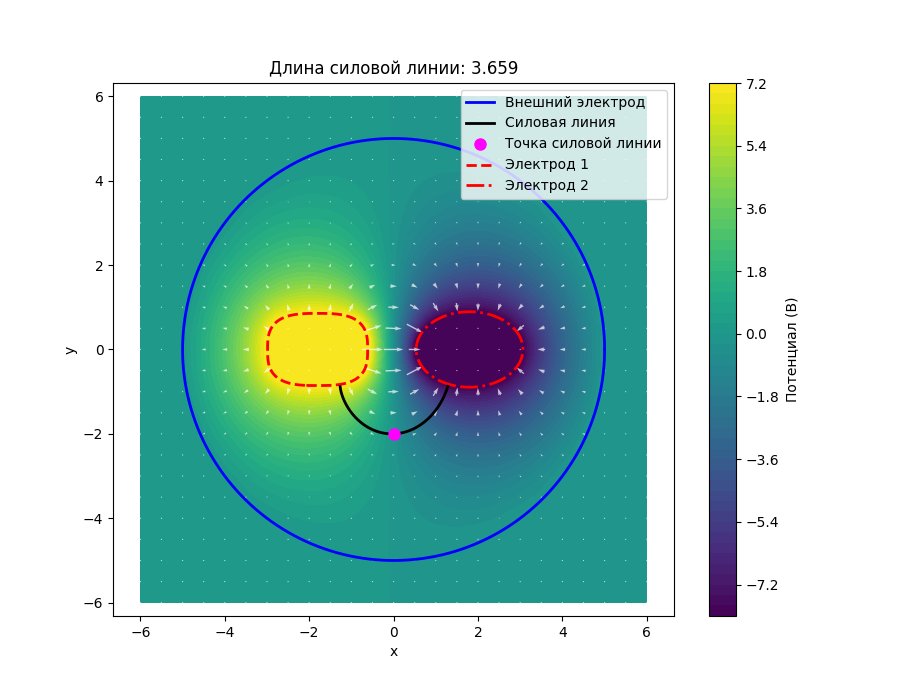
\includegraphics[width=0.75\textwidth]{pictures/result.png}
\end{center}
Для варианта 14 получена длина
\[
\text{Length} \approx 3.65900.
\]

%----------------------------------------
\section*{Выводы}
\begin{itemize}
  \item Перенос тяжёлых расчётов в C++ + SOR значительно ускорил решение и повысил точность.
  \item Малый шаг интегрирования \(ds=10^{-5}\) и билинейная интерполяция дали точность длины до \(10^{-5}\).
  \item Разделение на этапы (C++ → CSV → Python) упростило архитектуру и визуализацию.
\end{itemize}

\end{document}
